All experiments are computed on a 2018 MacBook Pro, with a 2.4 GHz Quad-Core
Intel Core i5 processor and 8GB of memory. Furthermore, data is stored to a
500 GB Apple solid state drive.

The performance impact of using \gls{JIT} compilation with Numba on top of Numpy
is illustrated in figure (\ref{fig:3_1_numba}). Here we benchmark the performance
of an implementation of insertion sort, an algorithm with an asymptotic complexity
bound of $O(N^2)$, when using an implementation built with Numpy containers and
compare this to an implementation using JIT compilation on top of Numpy containers.
Both functions are run five times on different inputs of the same size
in figure (\ref{fig:3_1_numba}). On larger problems it becomes apparent
that Numba offers an approximately constant speedup over Numpy, in fact for
sorting arrays of $10^4$ integers the JIT compiled function is $1050 \pm 80$
times faster than the pure Numpy function, where the error is provided to (1 s.f)
\footnote{Please refer to Appendix \ref{app:errors}, Section \ref{sec:app_numba},
for the specifics of the error propagation calculation in this experiment.}.

\begin{figure}[ht]
    \centering

  {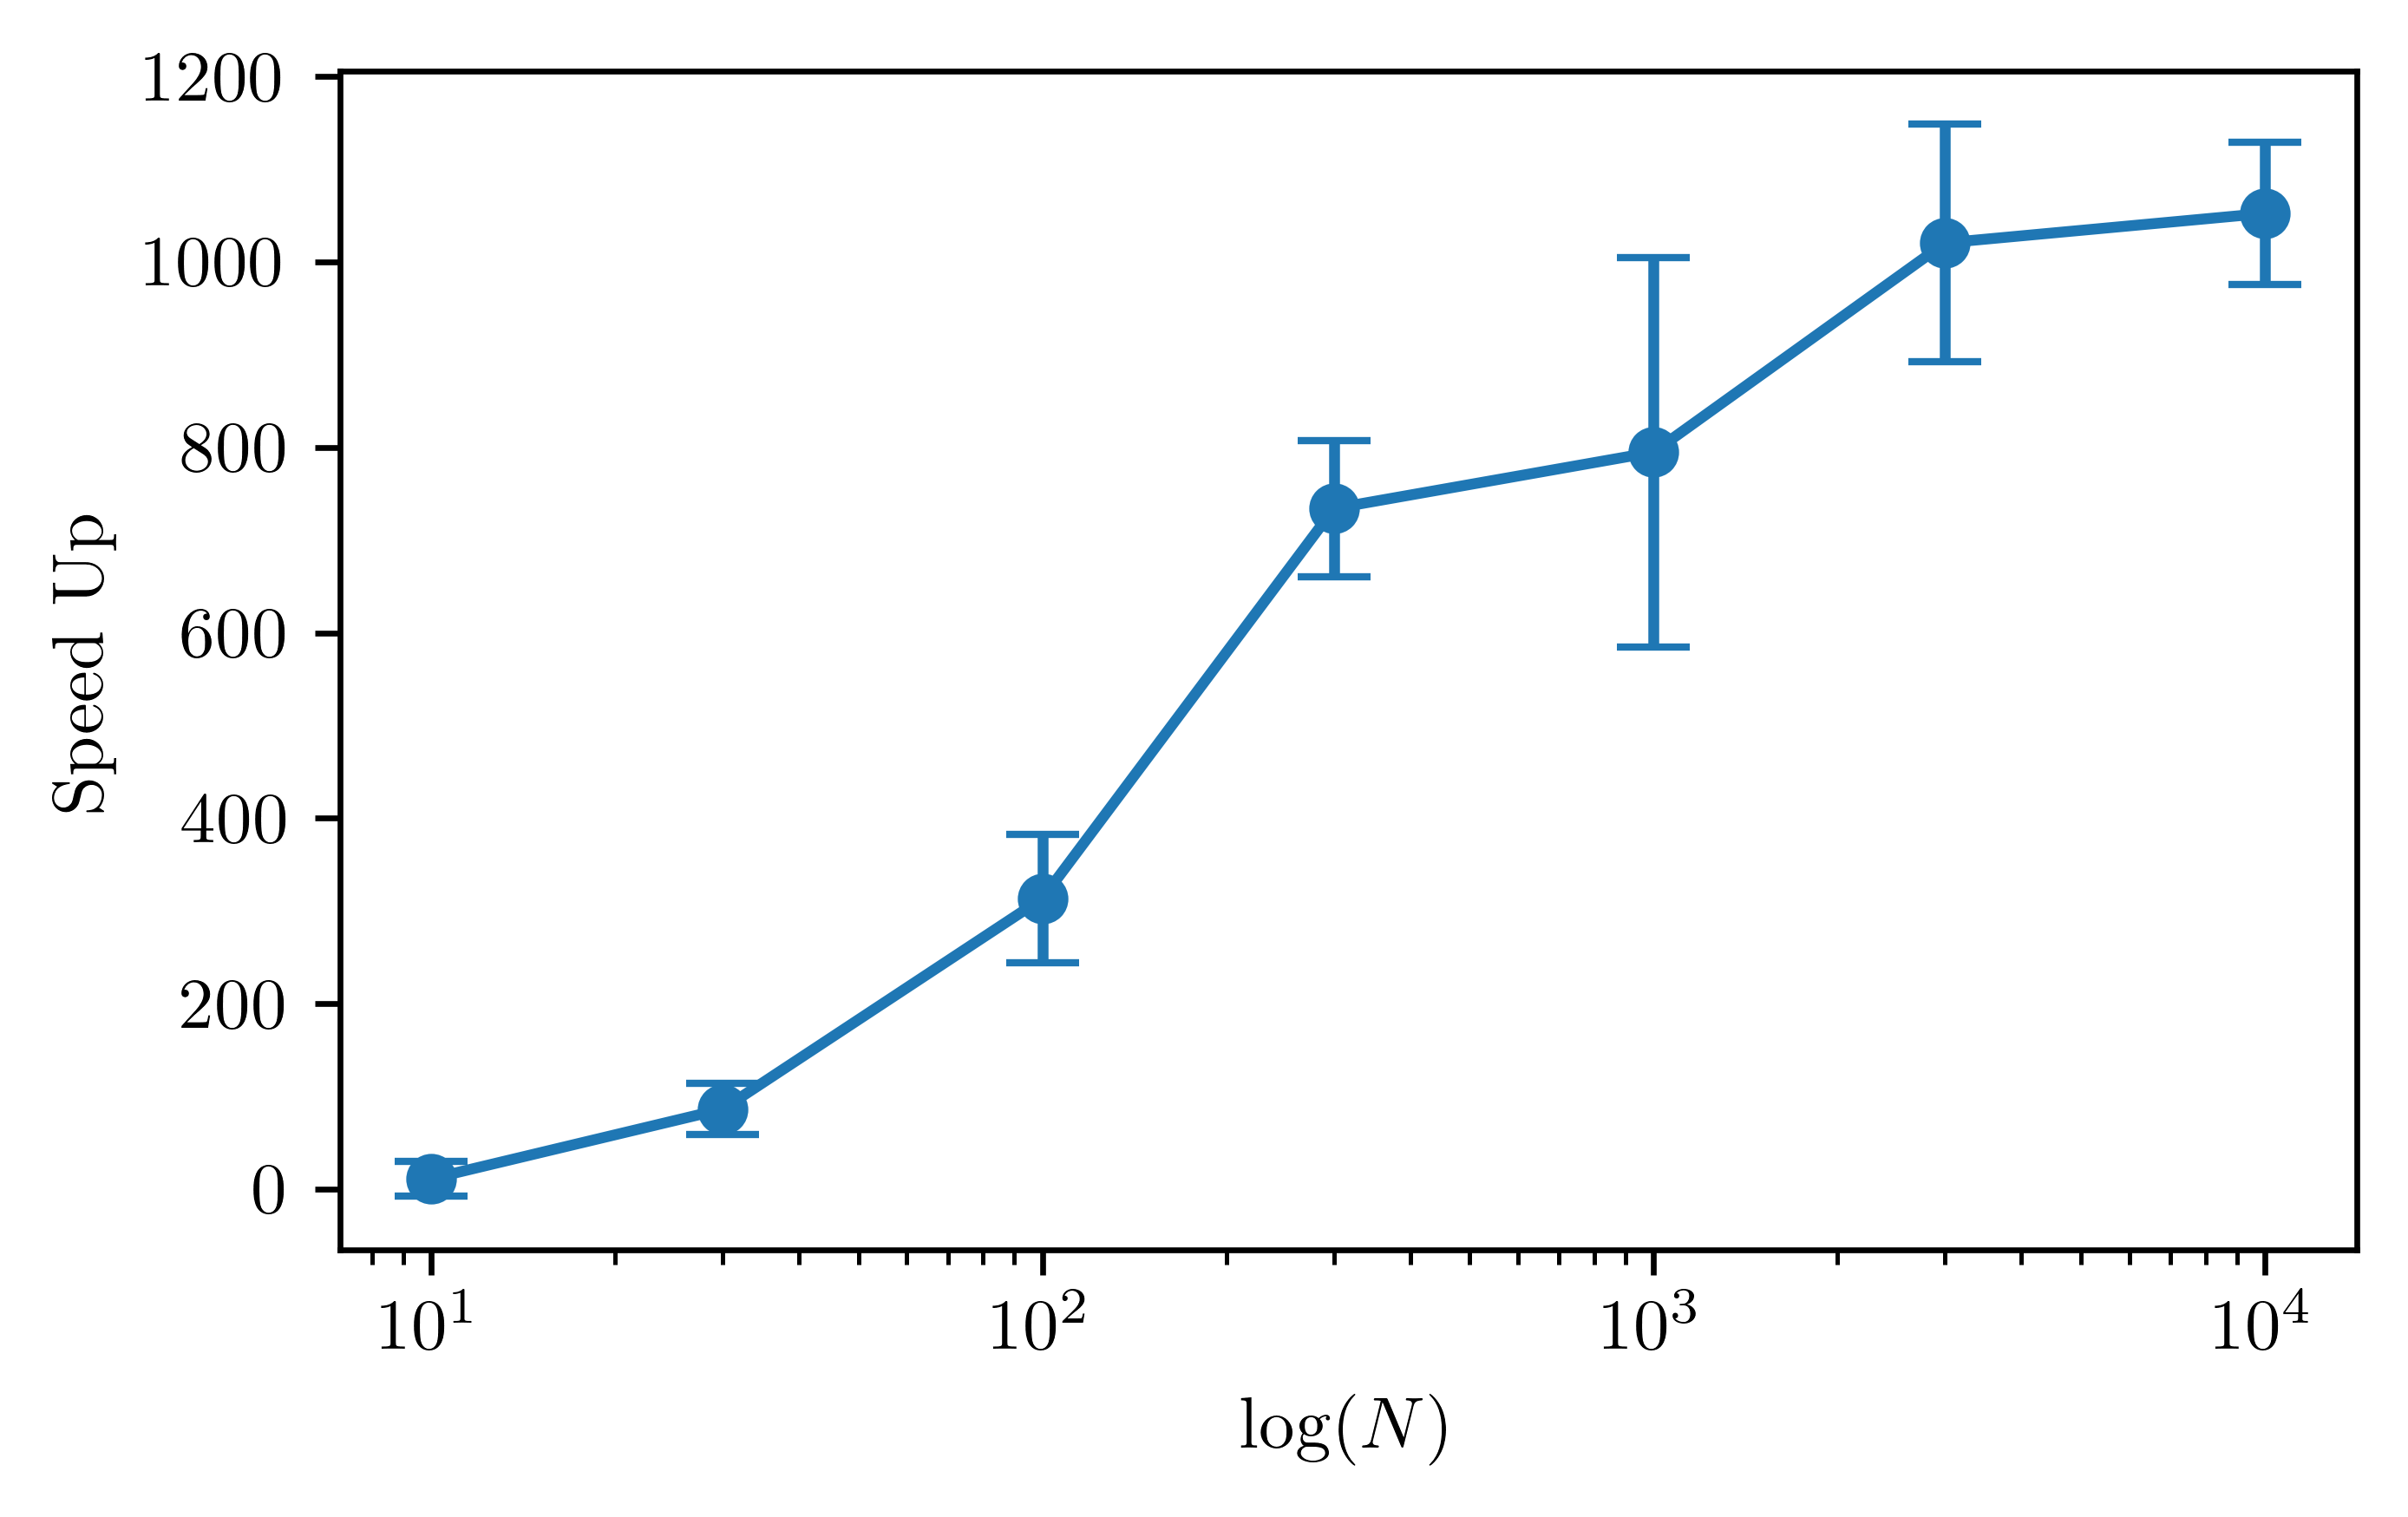
\includegraphics[width=0.9\textwidth]{chapter3/numba_speedup.png}}
  \vspace{0pt}
    \caption{The $y$ axis is the multiplicative speedup offered by using Numba in
    conjunction with Numpy for the above benchmarking experiment. The $x$ axis is
    the length of a list to be sorted $N$, plotted with a logarithmic scale. Error
    bars are plotted from the standard deviation in speedup over all trials.}
    \label{fig:3_1_numba}
\end{figure}

To benchmark the efficacy of HDF5 in comparison to serialisation for saving,
and loading data from disk we create a Numpy array composed of
20,000 columns and 10,000 rows of 64 bit floats. This array has a minimum size
of 1.5 GB (1 s.f.), excluding the metadata associated with the type, and is
saved and loaded 5 times from disk for statistics. Serialisation throughout
\gls{PyExaFMM} is computed using the core Python Pickle library. For saving,
serialisation takes $2.7 \pm 0.7$ seconds (1 s.f), and hdf5 takes $1.1 ± 0.2$ seconds (1 s.f).
For loading from memory, as HDF5's mechanism of returning a database style interface
rather than loading everything to disk, leads to the appearance of rapid
load times, we also measure the time taken to load the entire file to disk from
HDF5. Loading the serialised file takes $3.2 \pm 0.4$ seconds (1 s.f), loading
the HDF5 file to disk takes $1.4 \pm 0.1$ seconds (1 s.f). Using HDF5 is almost
twice as fast as serialisation, the reasons for this are due to the underlying
techniques used by each method. Roughly speaking, HDF5 stores raw numeric data
alongside a header file describing its dimensions, as a contiguous byte stream
on disk which allows for optimised methods to quickly search and retrieve data
\cite{collette2013python}. Object serialisation is designed to work with arbitrary
Python objects, raw numeric data is not stored, rather it is first compressed
into an intermediate representation, that results in a byte stream which is then
stored on disk. This data is stored alongside the metadata for the object, such
as it's initialisation code, and even any dependent objects it may have. The
intermediate representation allows any objects to be serialised in the same
manner \cite{pickle}.

Our model problem is the three dimensional electrostatic problem (\ref{eq:electrostatic_paradigm})
with the Laplace kernel. Due to the constraints of accessible computing power,
we benchmark the model performance, as well as the operator precomputation
calculations using, a 3 level non-adaptive octree, containing 1000 randomly distributed
particles which are used as sources as well as targets. All sources are given a
charge density of 1 Coulomb. Furthermore, the surfaces are calculated to order
$p=2$, therefore each discretised with $8$ quadrature points (\ref{eq:2_2_quadrature_points}), and the
parameters for the relative sizes of different surfaces are the same as those
provided in Chapter \ref{chpt:2_strategy_for_practical_implementation}, Section
\ref{sec:2_3_operator_caching}.

We benchmark the efficacy of multiprocessing for accelerating the precomputation
of the \gls{M2M}, \gls{L2L} and \gls{M2L} operator matrices for the above octree
using different numbers of CPU processor cores in figure (\ref{fig:3_1_multiproc}).
Precomputations are completed three times for a given number of processor cores,
for statistics. The speedup for increasing the number of processor cores is non-linear, this is
indicative of a communication overhead, and the fact that multiprocessing has
been implemented to a very basic degree with the required data being copied
over to each process, even if very large.

\begin{figure}[ht]
    \centering

  {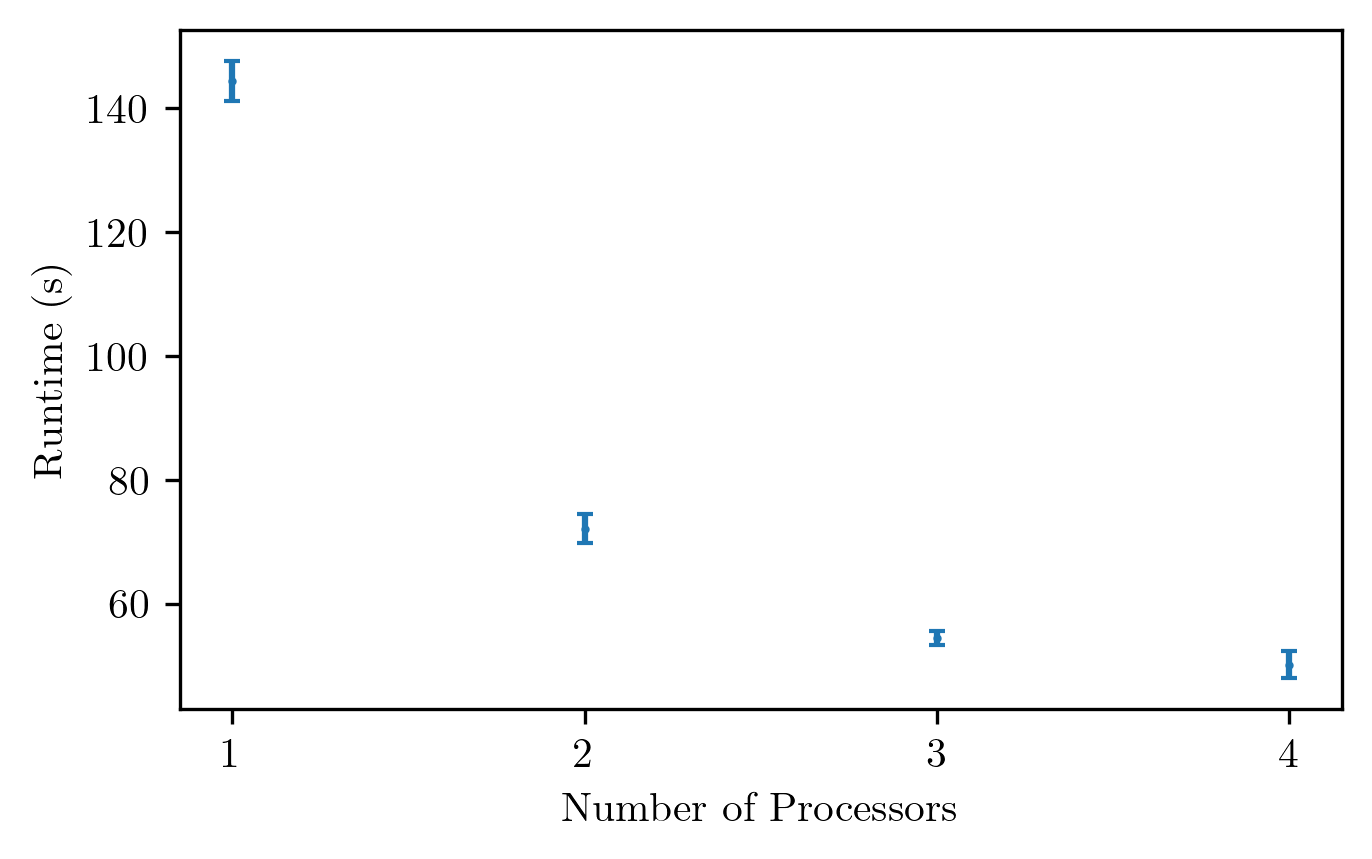
\includegraphics[width=0.9\textwidth]{chapter3/multiproc.png}}
  \vspace{0pt}
    \caption{Runtime versus number of processors used for operator precomputations.
    Error bars are plotted using standard deviation.}
    \label{fig:3_1_multiproc}
\end{figure}

We benchmark the algorithm run time in comparison to direct computation in figure
(\ref{fig:3_1_complexity}), with same parameters as the octree used for benchmarking
the operator precomputation, but with an increasing number of target and source
particles. The calculations are run three times for each input size $N$, for
statistics. Assuming a power relationship between run time $t$ and input size $N$,

\begin{equation}
    t = N^x
\end{equation}

where $x$ is unknown, taking logarithms allows one to apply least squares fitting
to fit a linear relationship to,

\begin{equation}
    \log(t) = x \log(N)
\end{equation}

computing the value of $x$ from the gradient. Performing this calculation for the
results from the \gls{FMM} and direct approaches we report $x=1.1$ (1 d.p) for
the FMM, and $x=2.0$ (1 d.p) for the direct method. This implies an asymptotic
complexity of $O(N^{1.1})$, and $O(N^2)$ for the \gls{FMM} and direct methods
respectively, with the limitation that this has been tested on relatively
small inputs of only $O(10^3)$ particles.

-\begin{figure}[ht]
    \centering

  {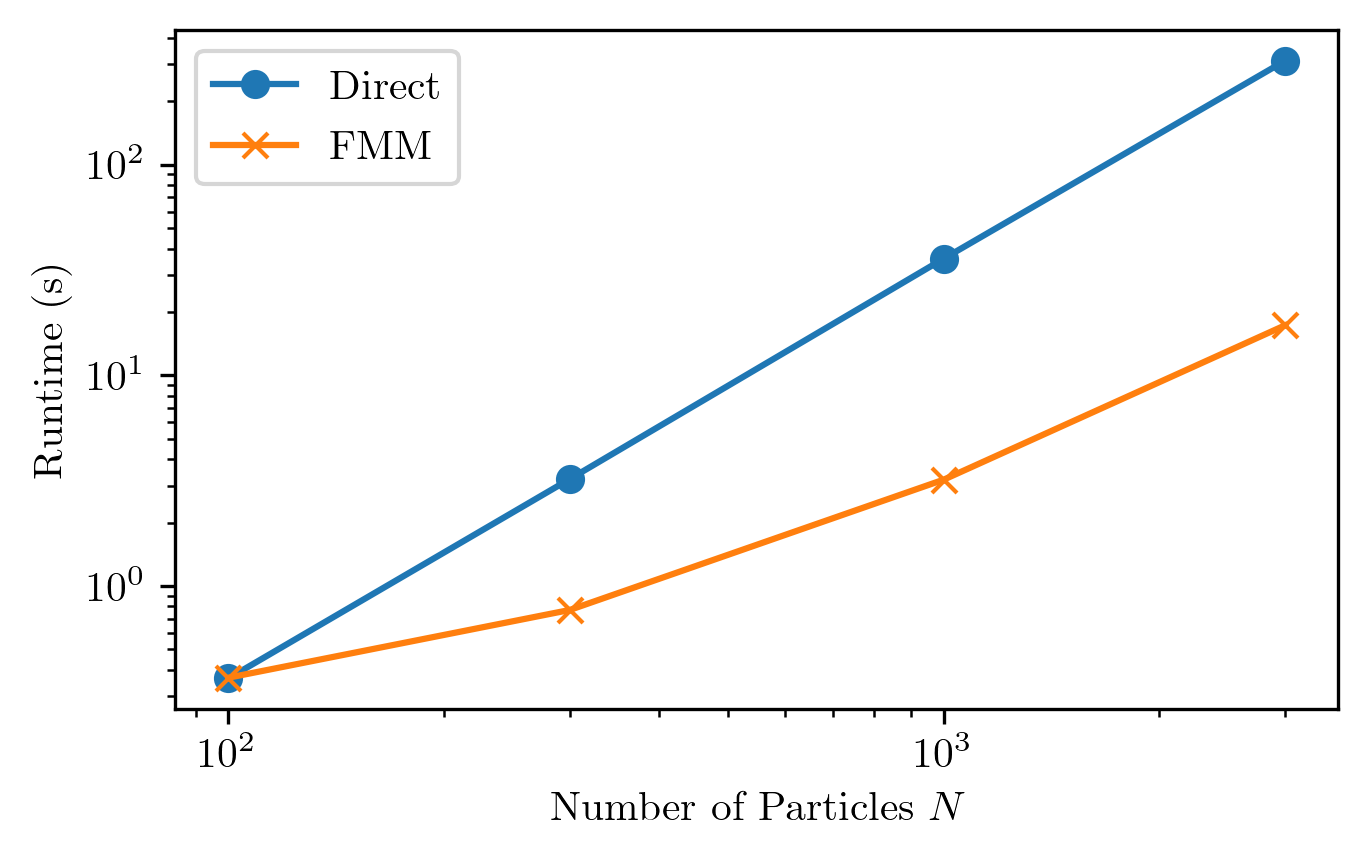
\includegraphics[width=0.9\textwidth]{chapter3/complexity.png}}
  \vspace{0pt}
    \caption{Foo Bar}
    \label{fig:3_1_complexity}
\end{figure}

- Understand cost of computation via pyexafmm compared to state of the art exafmm-t.

- Comment on where the slowness comes from

- no parallelism for operator evaluations

- no parallelism for memory sharing

- lots of copying of same data.

- subtoptimal data formats for m2l - lots of loading.

- suboptimal size of data structures lead to loading from non-cpu memory - which is slow - could be optimized via numexpr etc in the future or more intricate chunking of memory.

- These are justifiable from the time constraints on full-time development.

